% Para documento texto corto
%\documentclass[paper=letter,oneside,fontsize=12pt]{article}
\documentclass[paper=letter,oneside,fontsize=11pt, parskip=full]{scrartcl}
%\documentclass[paper=letter,oneside,fontsize=12pt]{scrartcl}

% Establece dimensiones de los margenes
% \usepackage[inner=1.5cm,outer=3cm,top=2cm,bottom=4cm,
% bindingoffset=5mm]{geometry}
\usepackage[left=3cm,right=3cm,top=3cm,bottom=3cm,
bindingoffset=0cm, footskip=0.5cm, headheight=2cm]{geometry}

% Elimina sangrias y aumenta espacio entre parrafos
\usepackage{parskip}

% Permite cambiar margenes derecho e izquierdo
% de secciones de texto con el entorno
% adjustwidth
\usepackage{changepage}

% Permite establecer el espaciado entre lineas
\usepackage{setspace}

% Permite ingresar caracteres acentuados y especiales 
% sin necesidad de emplear comando
% utf8 codificacion de entrada Unicode (mas simbolos que ASCII)
\usepackage[utf8]{inputenc}

% Formato direccione URL
% \usepackage{hyperref}

% T1 encoding for European, English, American text
\usepackage[T1]{fontenc}
% Fuente escalable
% \usepackage{lmodern}

% Reemplazo para fuente Arial
\usepackage{helvet}
% Usa la fuente sans-serif por defecto
\renewcommand{\familydefault}{\sfdefault}

% Carga babel, idioma ingles
\usepackage[english,spanish]{babel}

% Mejor jsutificacion, tipografia alta calidad.
\usepackage{microtype}
% Para unir columnas y filas en tablas
\usepackage{array}

% Agrega comandos extra al comando tabular
% \toprule, \midrule, \bottomrule
\usepackage{booktabs}
% Tablas con ancho establecido por usuario
\usepackage{tabularx}
% Para posicionamiento preciso de tablas dentro del texto
\usepackage{float}

% Encabezados personalizados
\usepackage{fancyhdr}
\usepackage{graphicx}

% Permite obtener el numero de la ultima pagina
\usepackage{lastpage}

% Paquetes para figuras
% Paquete caption para titulos figuras
% Paquete subcaption para subfiguras
\usepackage{caption}
\usepackage{subcaption}

% Espaciado inteligente
\usepackage{xspace} 

% Para formato de codigo fuente
\usepackage{xcolor}
\usepackage{listings}
\lstset{basicstyle=\ttfamily,
	showstringspaces=false,
	commentstyle=\color{red},
	keywordstyle=\color{blue}}

% Cabeceras
\pagestyle{fancy}
% Borra cabecera y pie actuales
\fancyhead{}
% Cintillo cabecera
%\chead{
%	
\includegraphics[width=150mm]{Imagenes/Cabecera.png}
%}
\fancyhead[L]{\includegraphics[width=0.3\textwidth]{Imagenes/cabecera.pdf}}
\fancyfoot[C]{ 
	\begin{tabularx}{\textwidth}{|m{3.0cm}|X|m{2.5cm}|m{1.0cm}|}
		\hline			
			\centering
			\includegraphics[height=0.8cm]{Imagenes/pie-izq.pdf} &			
			\centering
			Confidencial &
			\centering
			\includegraphics[height=0.8cm]{Imagenes/pie-der.pdf}  &			
			\thepage~/~\pageref{LastPage} \\
		\hline 
	\end{tabularx}	 
}

% Comando para formatear y justificar parrafos de código y 
% comandos de shell
% \newcommand{\code}[1]{
%	\begin{adjustwidth}{1.5cm}{0.0cm}
%		\ttfamily
%		#1
%	\end{adjustwidth}}	

% Entorno para formato de secciones de codigo
\newenvironment{code}
	{\begin{adjustwidth}{1.5cm}{0.0cm}\ttfamily}
	{\end{adjustwidth}}

% Entorno para formato de secciones de enlaces
\newenvironment{link}
	{\ttfamily}{}

% Numeracion de paginas
% numeros arabigos
\pagenumbering{arabic}

	\begin{document}
			
		%\begin{titlepage}
		
		\begin{center}		
			
			\vspace{10cm}
			% 12 puntos = fuente large
			\begin{large}
				\bfseries
				\uppercase{Dirección de Servicios de Certificación}			
				\vspace{5pt}
				\begin{spacing}{0.9}
					\uppercase{Laboratorio de Ensayos de Compatibilidad~Electromagnética~Radiada}
				\end{spacing}
			\end{large}
			
			%\vspace{10cm}
			\vfill
			
			% 16 puntos = fuente Large de 14 puntos			
			\begin{Large}
				\bfseries				
				\begin{spacing}{0.9}		
					\uppercase{Instalación de librería VXI-11}
				\end{spacing}
			\end{Large}	
				
			\vspace{5pt}
			
			% 12 puntos fuente large
			\begin{large}						
				\uppercase{Sub Título}
			\end{large}	
			
			\vfill
			
			\begin{table}[!h]
				\begin{tabularx}{\linewidth}{|X|X|X|X|}	
					\hline				
					\multicolumn{2}{|l|}{\textbf{CÓDIGO}: FO-IT-002} & \multicolumn{2}{l|}{\textbf{N DOC:}} \\
					\hline
					Originado por:	& 	Elaborado por: & 
					Revisado por: 	& 	Aprobado por: \\
					\hline
					Br. Arias B., Jose A. & Br. Arias B., Jose A. & - & - \\
					\hline
					\textbf{Fecha: 07/07/2017 } & 
					\textbf{Fecha: 07/07/2016} & 
					\textbf{Fecha: } &
					\textbf{Fecha: } \\				
					\hline
				\end{tabularx}	
			\end{table}	
			
			%\vspace{10mm}			
			\vfill
		
		\end{center}
	
	%\end{titlepage}
	
	\clearpage
	
	\tableofcontents
	
	\section{Objetivos}
		\begin{itemize}
			\item Describir el acceso a instrumentos de medición por medio del puente LAN/GPIB E5810
		
		\end{itemize}
		
	\section{Alcance}
	
		En este documento se explica como establecer un puente de conexión entre instrumentos de medición GPIB y una red LAN. Para ello se estblecerá la configuración del puente LAN/GPIB Agilent E5810A. Se detallará principalmente la instalación de la libreria VXI-11 para linux, soporte de software que permite el acceso programático a este dispositivo.	
		
	\section{Documentos de referencia}
	
		\subsection{Enlances de interés}

	
			\begin{link}

			\end{link}	
	

	
	\section{Términos y definiciones}
	
		\begin{tabular}{rl}
			Termino 	& 	Definición \\	
			VXI			& 	VMEbus eXtensions for Instrumentation \\
			RPC			& 	Remote Procedure Call \\
		\end{tabular}
	
	\section{Personal autorizado}	
		\label{Sec:PersonalAutorizado}		
		Personal técnico del Cendit con interés en el acceso a instrumentos de medición GPIB por medio de un puente de redes LAN a GPIB.
		
	\section{Personal requerido}	
		
		Ver sección \ref{Sec:PersonalAutorizado}.
		
	\section{Materiales}
	
		\label{Sec:SeccionMateriales}
		\begin{itemize}
			\item Computador con acceso a internet.
			\item Puente LAN/GPIB Agilent E5810A.
			\item Cable ethernet cruzado.
		\end{itemize}	
			
	\section{Herramientas y equipos}
		
		Ver sección \ref{Sec:SeccionMateriales}.

	
	\section{Equipos de protección personal}
	
		No se requieren equipos protección personal.
		
	\section{Precauciones de seguridad}
	
		Para ejecutar esta actividad no se preveen precauciones de seguridad
		
	\section{Descripción de la actividad}
	
		\subsection{Generalidades}		

		La especificación \emph{VXI-11} fue desarrollada a comienzos de los años 90 como una parte de una especificación mayor, la del bus \emph{VXIbus}. VXI-11 define el protocolo de comunicaciones por medio del cual instrumentos de medición y controladores se comunican sobre una red TCP/IP. 
		
		Fue empleada en puentes LAN/GPIB antes de que existiesen los instrumentos con una interfaz LAN nativa. 	Un punto importante de la especificación VXI-11 es la de lograr la interconexión de dispositivos de manera independiente de su fabricante.			
		
		Las comunicación y el paradigma de  programación es similar a los soportados por los estándares IEEE-488.1 e IEEE-488.2 en el sentido de que las comunicaciones son basadas en transferencia de datos ASCII y mensajes de control IEEE-488.1, entre un controlador y un dispositivo, sobre una red de computadores. Esto se debe a que	VXI-11 fue ideada en principio para replicar ciertas características de un bus GPIB a una red LAN, incluyendo aquellas características propias del hardware (señalización del bus). 
				
		Esta especificación posee tres sub secciones, VXI-11.1 trata la interconexión de dispositivos VXIbus a una red. VXI-11.2 trata la conexión de instrumentos GPIB a una red por medio de puentes Lan a GPIB como el Agilent E5810A, VXI-11.3 trata de la conexión de instrumentos que cumplen con el estándar IEEE-488, y que poseen una interfaz Ethernet para conexión directa a una red Lan.
		
		Las comunicaciones dentro de la especificación VXI-11 se efectúan sobre el protocolo ONC Remote Procedure Call (RPC). El protocolo  RPC permite un enlace de tipo cliente-servidor, una aplicación (típicamente el cliente) efectúa llamadas a procedimientos en una aplicación remota (el servidor), como si estos procedimientos remotos fuesen ejecutado localmente. 
		
		RPC fue diseñado para ser independiente de un lenguaje de programación, sistema operativo o plataforma de computador en particular, el servidor RPC y el cliente RPC pueden ejecutarse en diferetes sistemas operativos y procesadores.  Esta \emph{interoperabilidad} se logra al representar los datos que viajan por la red en el formato XDR, el cual define tipos de datos estándar y el ordenamiento de los bytes de datos empleados en las llamadas RPC. 
		
		Cuando se realiza una llamada a un procedimiento RPC, los datos  que se pasan a una función deben traducirse del formato del lenguaje de programación utilizado al formato XDR y en el servidor se traducen de vuelta, de XDR al formato nativo del lenguaje de programación.
		
		Las funciones disponibles en un servidor RPC se describen por medio de un archivo RPCL (RPC Language). La definición de funciones en el archivo RPCL es muy similar a la definición de tipos  C.		
		
		En la figura se muestran las funciones RPC para uso con VXI-11 y se muestra una entrada que describe estas funciones en el archivo RPCL.
				
		\begin{figure}[!h]
			\begin{center}
				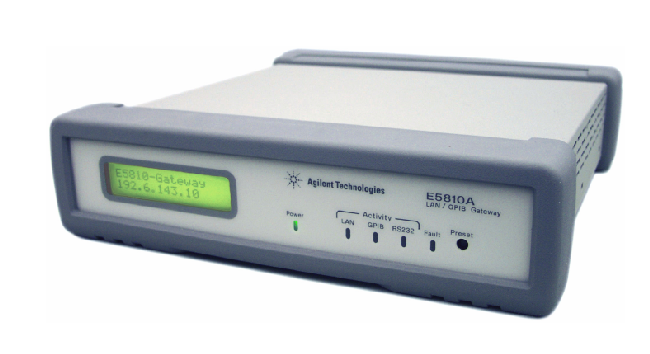
\includegraphics[width=10cm]{Imagenes/E5810.pdf}
				\caption{Puente LAN/GPIB E5810 de Agilent Technologies}
				\label{Fig:PuenteLanGpib}				
			\end{center}
		\end{figure}
	
		\begin{figure}
			\begin{lstlisting}[language=c]	
program DEVICE_CORE { 
	version DEVICE_CORE_VERSION { 
		Create_LinkResp create_link (Create_LinkParms) = 10; 
		Device_WriteResp device_write (Device_WriteParms) = 11; 
		Device_ReadResp device_read (Device_ReadParms) = 12; 
		Device_Error destroy_link (Device_Link) = 23; 
	} = 1; 
} = 0x0607AF;	
			\end{lstlisting}
		\end{figure}
		
		El sistema operativo brinda el soporte necesario para la transferencia de datos sobre RPC, en forma de librerías. Por ejemplo la función clnt\_call() del sistema operativo permite llamar a funciones RPC, aunque su uso es tedioso. Una forma de facilitar las llamadas RPC es por medio de una utilidad llamada rpcgen, la cul toma el archivo de definición de funciones RPCL del servidor y crea un conjunto de archivos con funciones de C, los cuales crean una capa de software que facilita las llamadas a funciones y la conversion de datos a XDR.
		
		\subsection{Librería VXI}
		Es una compilación de código fuente que permite establecer comunicación con instrumentos habilitados para ethernet y que usen el protocolo VXI11, para Linux. Permite la comunicación con una amplia gama de instrumentos como osciloscopios, analizadores logicos generadores de funciones. Incluye además dos utilidades interactivas para enviar y reibir comandos SCPI a los instrumentos.
		
		El autor del código, Steve D. Sharples, logró conseguir los archivos RPCL originados de la especificación del protocolo VXI-11. 
		
		\subsubsection{Archivos componentes}
		La librería consiste en los siguientes archivos de código fuente:
		
		\begin{description}
			\item[\ttfamily vxi11.x] el cual es una fusión de los archivos RPCL vxi11core.rpcl y vxi11intr.rpcl. Es una base ligera para vxi11 sobre rpc. Si se ejecuta rpcgen en este archivo, se generan los archivos de C y cabeceras, a partir de los cuales se pueden escribir programas de C para comunicación con instrumentos ethernet. Al ejecutar la utilidad \texttt{rpcgen} sobre este archivo, se genera los archivos de C con sus respectivas cabeceras los cuales contienen las funciones necesarias (ver tabla \ref{Tab:FuncionesVXI11Basicas}) para establecer comunicación con instrumentos mediante el protocolo RPC.
			
			\item[\ttfamily vxi11\_user.cc y vxi11\_user.h]  incluye varias funciones, entre ellas 4 funciones clave para facilitar la programación al usuario: xi11\_open(), vxi11\_close(), vxi11\_send() and vxi11\_receive(). Incluyen funciones que encapsulan la complejidad de las llamadas nativas RPC.
			
			\item[\ttfamily vxi11\_cmd.c] código fuente para utilidad interactiva de linea de comando llamada \texttt{vxi11\_cmd} que permite enviar comandos y consultas a un instrumento vxi11, el cual se localiza por medio de su dirección IP.
			
			\item[\ttfamily Makefile] archivo con guio de instrucciones par la utilidad make, que permite construir el programa utilidad vxi11\_cmd. Simplemente se teclea make para compilar el codigo. Luego make clean para eliminar antiguo archivos con codigo objeto (.o) y ejecutables. Por ultio con make install se copia la utilidad vxi11\_cmd a /usr/local/bin.		
		\end{description}		
	
		\begin{table}
			\begin{tabular}{cl}
				\textbf{Función API} 	& \textbf{Descripción} \\
				\texttt{create\_link}	& Establece un enlace a un dispositivo lógico dentro de un servidor VXI-11 \\
				\texttt{device\_write}	& Envía un comando (típicamente SCPI) a un instrumento \\
				\texttt{device\_read}	& Lee datos de un instrumento \\
				\texttt{destroy\_link}	& Libera el enlace establecido por \texttt{create\_link} y libera los recursos utilizados.				
			\end{tabular}
			\caption{Funciones VXI-11 básicas}
			\label{Tab:FuncionesVXI11Basicas}
		\end{table}
	
	\subsubsection{Utilidades}
	
	Dentro del código fuente se encuentra el archivo de nombre \texttt{Makefile}. Este archivo sirve de entrada para el comando \texttt{make} de linux, el cual permite generar la utilidad \texttt{vxi11\_cmd}, de la siguiente manera,
	
	\begin{code}
		make clean \\
		make install		
	\end{code}
	
	La primera instrucción permite remover antiguos archivos de código objeto de construcciones previas. El último comando permite construir la utilidad \texttt{vxi11\_cmd} y copiarla a la ruta \texttt{/usr/local/bin}.	
	
	\subsection{Construcción de la librería libvxi11.so}	
	
	El código fuente incluye el archivo \texttt{makefile} que le permite al comando \texttt{make} generar un ejecutable  \texttt{vxi11\_cmd} , una utilidad de depuración que sirve para enviar y recibir comandos textuales (scpi) a un instrumento.

	Si se desea emplear el código fuente en una aplicación que requiere la comunicación con instrumentos LAN, el programador o 
	desarrollador tiene dos opciones.
	
	\begin{enumerate}
		\item Integrar el código fuente a la aplicación. 
		\item Generar una librería a partir del código fuente y enlazar la librería con la aplicación.
	\end{enumerate}	

	La opción 1 es la más simple siempre y cuando se desarrolle una aplicación en leguaje C/C++. Solo requiere incluir dentro del código fuente de la aplicación a desarrollar los archivos \texttt{vxi11.h}, \texttt{vxi11\_user.h} y \texttt{vxi11\_user.cc}, que forman parte del código fuente para VXI-11. El programador podrá emplear las funciones básicas de la que se muestran en la tabla \ref{Tab:FuncionesVXI11Basicas}. La aplicación se ebe compilar como un todo.
	
	La opción 2 permite generar una librería que contenga las funciones de comunicación y a la cual la aplicación puede cargar al momento de iniciar la ejecución. Presenta la ventaja que se compila y construye el código fuente VXI11 sólo una vez, cuando se construye la librería. Además es posible llamar a las funciones de esta librería escrita en C/C++ desde otros lenguajes de programación, como Java, C\# (CSharp) o Python.
	
	En linux, se pueden generar dos tipos de librería: estática o dinámica. Una librería estática es un archivo con extensión \texttt{.a}, esta se incluye como parte del programa durante la \emph{compilación}. Es el equivalente a un archivo \texttt{.lib} en Windows.
	
	Una \emph{librería dinámica de objetos compartidos (shared objects)} es un archivo con extensión \texttt{.so} se construye aparte de la aplicación principal y se carga cuando arranca la aplicación.
	
	Para generar la librería \texttt{libvxi11.so} se empleará el archivo de código fuente \texttt{vxi11\_user.cc} el cual incluye las funciones de usuario necesarias para establecer comunicación VXI11 con los instrumentos Lan. Este archivo requiere los archivos de cabecera fuente \texttt{vxi11\_user.h} y \texttt{vxi11.h}. 
	
	El archivo \texttt{vxi11\_user.cc} es un archivo de C++, ya que presenta funciones sobrecargadas, esto es, funciones con el mismo nombre pero con distintos numero y tipo de parámetros. La librería debe generarse con el compilador de C++ de linux, \texttt{g++}.
	
	El compilador de C++ genera una especie de transformación en los nombres de las funciones que se conoce como \emph{decoración de nombres} o \emph{name mangling}. Simplemente el compilador le agrega un prefijo al nombre de la función que indica el numero y tipo de argumentos que recibe la función. Esto lo realiza para permitir funciones con el mismo nombre pero distintos argumentos, es decir, la sobrecarga de funciones.  
	
	Por ejemplo, el nombre de la función \texttt{int	vxi11\_open\_device(const char *ip, CLINK *clink, char *device) } es codificado por el compilador g++ como 
	
	\begin{code}
		\_Z15vxi11\_open\_linkPKcPP6CLIENTPP15Create\_LinkRespPc	
	\end{code}

	Si se pretende realizar llamadas a las funciones de la librería desde un lenguaje de programación como Java, es conveniente utilizar los nombre sin decoración, es decir los nombres de las funciones tal como se escriben en los archivos fuente. Para ello se agrega el especificador \texttt{extern "C"}
	

	\begin{code}
		g++ vxi11_user.cc  -Wall -shared -o libvxi11.so
	\end{code}
	
	

	

	
	
	
	
			
	\section{Anexos}	
		
		\subsection{Script de Bash para carga automática de firmware}
	
			\begin{lstlisting}[language=c,caption={Listado programa}]
	
#include <stdlib.h>
#include <stdio.h>

int main()
{
	printf("Hola Gafo");
	
	return 0;
}
{}
		\end{lstlisting}
\end{document}